\chapter{The Solution}

The purpose of this chapter is to clearly identify, discuss, and justify the decisions you make
Depending on your type of project, you may not need to include all of these:


\section{Architectural Level}

\begin{figure}[h]
    \centering
    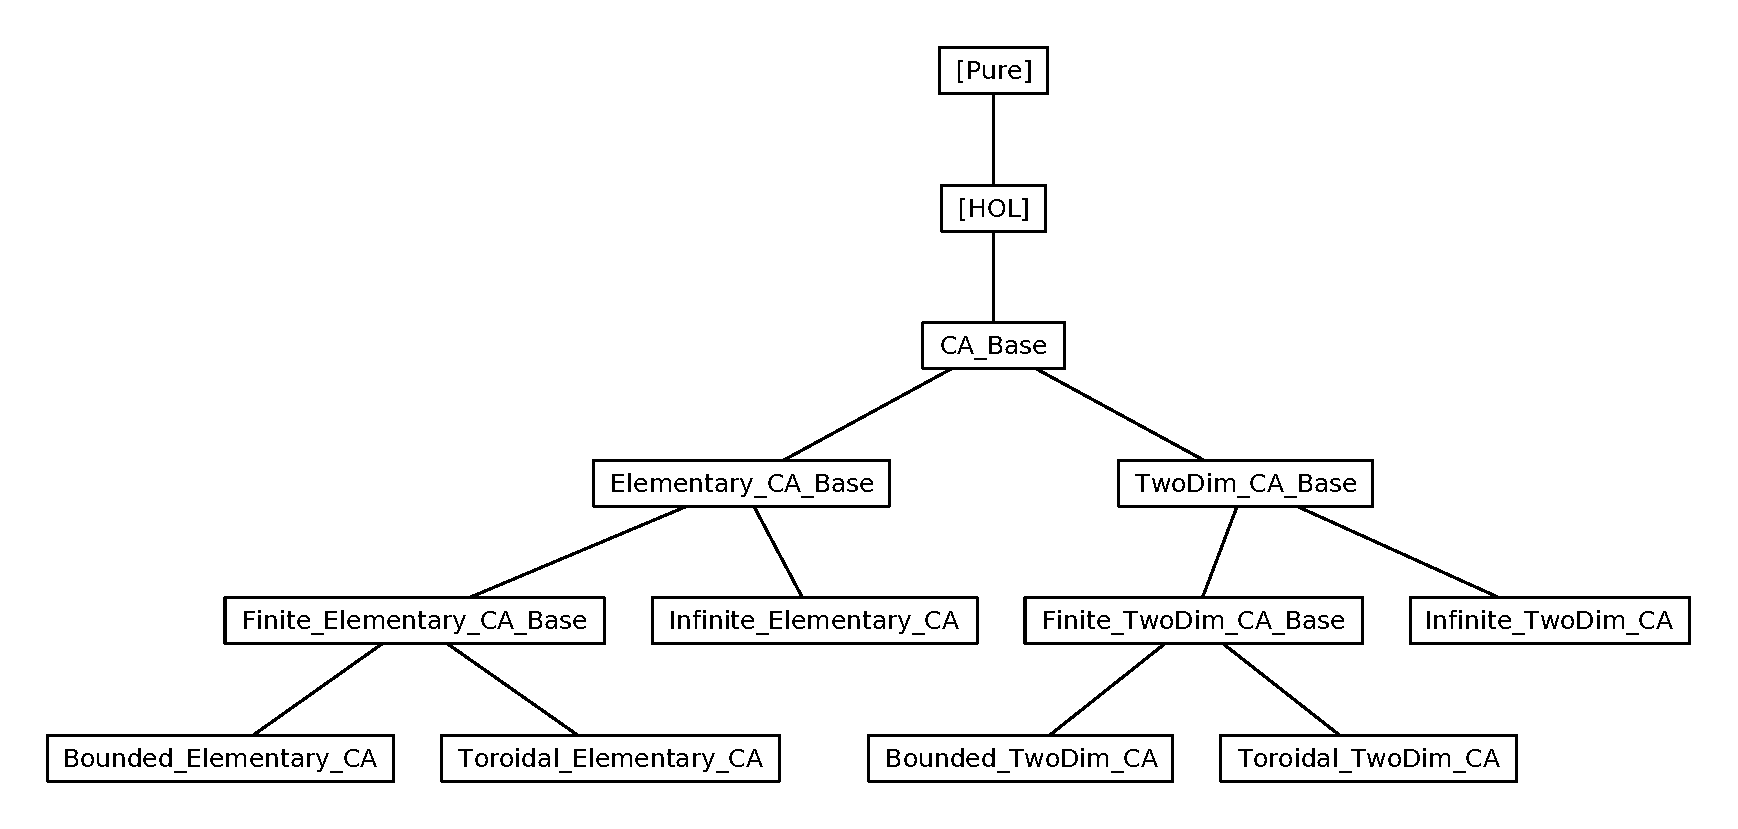
\includegraphics[scale=0.62]{session_graph.pdf}
    \caption{Dependency graph of project Theories}
    \label{fig:graph}
\end{figure}

\Cref{fig:graph} represents the overall architecture of dependencies of the various theory files in the project,
with files further down the tree depending on those above.
\mintinline{isabelle}{[Pure]} and \mintinline{isabelle}{[HOL]} contain the base definitions necessary to do work in Isabelle,
all the rest are new theories created for the project.

From the simplest core definitions given in \mintinline{isabelle}{CA_Base},
the project essentially splits into two due to the differences in implementing one dimensional versus two dimensional CA.
However the internal structure of these two subtrees are exactly the same apart from the distinction in dimension.
They both contain a base file for the two kinds of finite CA,
and another file dealing with the infinite case.

Each of the six root nodes contains the definition of one of the six distinct kinds of CA realised in the project.
They very roughly increase in power and complexity from left to right.

\section{The Cellular Automata Type}

The type of \mintinline{isabelle}{Cellular Automata} is redefined for each of the four main branches in the project.
Those are elementary finite,
two-dimensional finite,
elementary infinite,
and two-dimensional infinite.
This is due to the geometric and functional differences that have to exist in the \mintinline{isabelle}{state} type parameter underlying each broad class of CA.
Despite this, the actual signature of the type remains unchanged for each.
This is the allow the definitions and proofs that sit on top of them to make the same assumptions about type structure and composition.
As shown below in \Cref{code:ca_def} the definition is very compact and simple.
All CA also share the binary cell type given in \Cref{code:cell_def}.

As you would hope,
a Cellular Automata consists only of the current global state it is in,
and the rule necessary to transition it to the next state.
This however does hide quite a lot of complexity,
and in fact the actual functioning of a CA is created from more than these two parameters.

As an example of this,
\cite{yu} actually defines CA as a 4-tuple $(k, S, N, f)$,
where $k$ is the dimension,
$S$ the set of states,
$N$ the neighbourhood,
and $f$ the local rule.
This is certainly more transparent then the definition given here.
In this project's version the information about neighbourhoods is given implicitly from a neighbourhood function that sits in the local context where we want to actually run the CA.
The reason for the approach taken here is for elegance and ease of use in further results on the CA type.
Adding more information to the type directly can mean more work in pattern matching,
and constructing and deconstructing the type every time it is used.

\begin{myminted}{Cell definition}{cell_def}
    datatype cell = Zero | One
\end{myminted}

\begin{myminted}{CA type signature}{ca_def}
    datatype CA = CA (State : state) (Rule : rule)
\end{myminted}

The \mintinline{isabelle}{State} and \mintinline{isabelle}{Rule} that are capitalised are just syntactic sugar for defining accessor functions for those arguments to the type.
So the \mintinline{isabelle}{State} function takes a CA and returns its state, 
and similar for \mintinline{isabelle}{Rule}.

It is also worth noting that the CA here is not directly defined as a tuple.
Using a unique datatype carries more semantic weight then giving a \mintinline{isabelle}{type_synonym} to a tuple.
The same concept does not exist in general mathematics so purely mathematical approaches to formalisms usually just involve a tuple.


\subsection{State}

As mentioned in the above paragraphs,
the \mintinline{isabelle}{state} type is designed differently across the four general distinctions of CA.
As such the more detailed description of each is left to its own respective section.
For a high level overview it suffices to say that the finite CA states were simply a one or two dimensional list of states,
given geometry through either pattern matching or indices.
The infinite CA states were modeled completely differently,
as a function from the integers to cells.

\subsection{Neighbourhoods \& Rules}

Unlike \mintinline{isabelle}{state},
\mintinline{isabelle}{rule} is defined exactly the same way for all CA, as given in \Cref{code:rule_def}.
The only differing factor being the type of neighbourhood it acts on.

\begin{myminted}{Type definition of \mintinline{isabelle}{rule}}{rule_def}
    type_synonym rule = "neighbourhood => cell"
\end{myminted}

Neighbourhoods differ between one and two dimensions as expected but not in a conceptually deep way.
As shown in \Cref{code:nb_def} the only practical difference is adding more \mintinline{isabelle}{cell} arguments.

\begin{myminted}{The two kinds of neighbourhood}{nb_def}
    (* One dimensional *)
    datatype neighbourhood = Nb cell cell cell

    (* Two dimensional *)
    datatype neighbourhood = Nb
    (NorthWest:cell) (North:cell)  (NorthEast:cell)
    (West:cell)      (Centre:cell) (East:cell)
    (SouthWest:cell) (South:cell)  (SouthEast:cell)
\end{myminted}

\section{Finite Cellular Automata}

There ended up being two separate paths taken in dealing with the cells on the boundary of the finite CA.
The first,
which for the purposes of the project is named \emph{bounded},
is the simplest conceptually,
but not necessarily in implementation.

Bounded CA deal with the problem of determining the neighbourhood of a cell on the edge simply via ``padding''.
For the purposes 








\section{Analytical Work}

E.g. Equations, etc. that describe your solution


\section{Low Level}

E.g. Method specifications, Algorithms, etc.


\section{Implementation}

Discuss anything interesting here; put full source code in an appendix or attachment
